
%(BEGIN_QUESTION)
% Copyright 2013, Tony R. Kuphaldt, released under the Creative Commons Attribution License (v 1.0)
% This means you may do almost anything with this work of mine, so long as you give me proper credit

Suppose an operator tells you that the pH reads below 4.0 in this system, despite having checked the actual pH of the process water as approximately 7.3 pH using a ``grab sample'' tested with a benchtop pH meter.  Identify possible faults which could account for this incorrect reading:

$$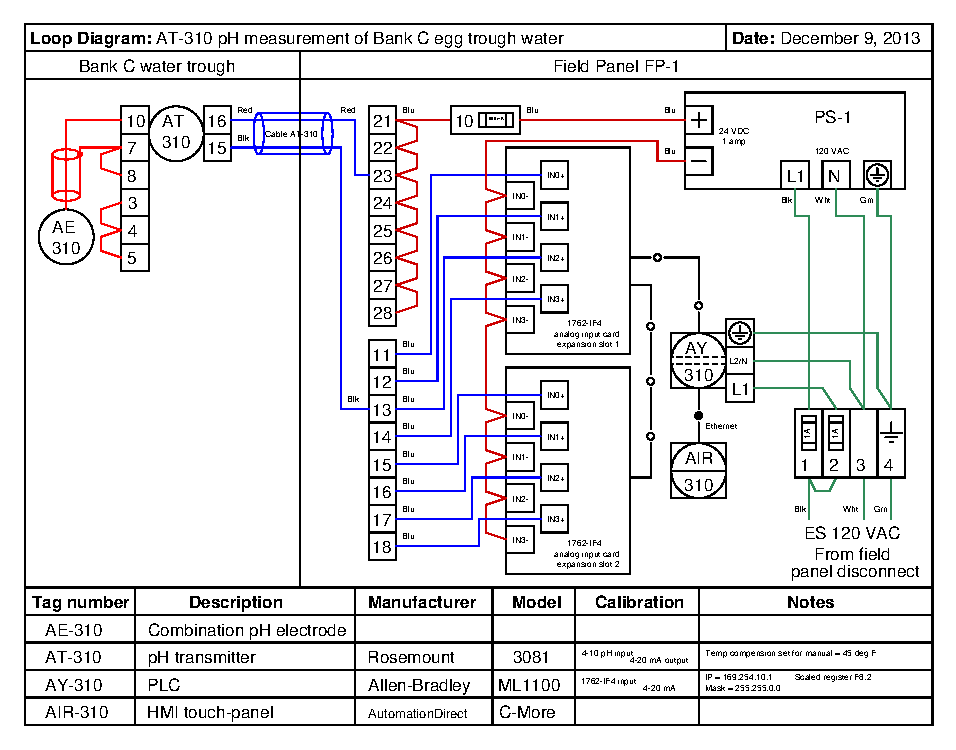
\includegraphics[width=15.5cm]{i0017rx02.eps}$$

\underbar{file i03082}
%(END_QUESTION)





%(BEGIN_ANSWER)

This symptom is indicative of an open wire somewhere in the 4-20 mA loop circuit.  Many faults are possible here.

%(END_ANSWER)





%(BEGIN_NOTES)

\filbreak \vskip 20pt \vbox{\hrule \hbox{\strut \vrule{} {\bf Virtual Troubleshooting} \vrule} \hrule}

\noindent
{\bf Predicting the effect of a given fault:} present each of the following faults to the students, one at a time, having them comment on all the effects each fault would produce.

\begin{itemize}
\item{} 
\item{} 
\item{} 
\end{itemize}


\vskip 10pt


\noindent
{\bf Identifying possible/impossible faults:} present symptoms to the students and then have them determine whether or not a series of suggested faults could account for all the symptoms, explaining {\it why} or {\it why not} for each proposed fault:

\begin{itemize}
\item{} Symptom: {\it }
\item{}  -- {\bf Yes/No}
\item{}  -- {\bf Yes/No}
\item{}  -- {\bf Yes/No}
\end{itemize}


\vskip 10pt


\noindent
{\bf Determining the utility of given diagnostic tests:} present symptoms to the students and then propose the following diagnostic tests one by one.  Students rate the value of each test, determining whether or not it would give useful information (i.e. tell us something we don't already know).  Students determine what different results for each test would indicate about the fault, if anything:

\begin{itemize}
\item{} Symptom: {\it }
\item{}  -- {\bf Yes/No}
\item{}  -- {\bf Yes/No}
\end{itemize}


\vskip 10pt


\noindent
{\bf Diagnosing a fault based on given symptoms:} imagine the AC power fuse on terminal 1 blows (i.e. fails open) in this system (don't reveal the fault to students!).  Present the operator's observation(s) to the students, have them consider possible faults and diagnostic strategies, and then tell them the results of tests they propose based on the following symptoms, until they have properly identified the nature and location of the fault:

\begin{itemize}
\item{} Operator observation: {\it pH measurement registered on AIR-310 is below 4.0 pH}
\item{} $V_{16-15}$ = 0 volts DC
\item{} $V_{IN2+-IN2-}$ = 0 volts DC
\item{} $V_{+-21}$ = 0 volts DC
\item{} $V_{supply output}$ = 0 volts DC
\item{} $V_{supply input}$ = 0 volts AC
\item{} $V_{PLC supply}$ = 119 volts AC
\item{} $V_{10-7}$ = 0 volts DC
\end{itemize}

%INDEX% Documentation, loop diagram: realistic industrial example (Perry Center salmon hatchery PLC field panels)

%(END_NOTES)


